% \iffalse meta-comment
%
% Copyright (C) 2017--2020 by Xiangdong Zeng <xdzeng96@gmail.com>
%
% This work may be distributed and/or modified under the
% conditions of the LaTeX Project Public License, either
% version 1.3c of this license or (at your option) any later
% version. The latest version of this license is in:
%
%   http://www.latex-project.org/lppl.txt
%
% and version 1.3 or later is part of all distributions of
% LaTeX version 2005/12/01 or later.
%
% This work has the LPPL maintenance status `maintained'.
%
% The Current Maintainer of this work is Xiangdong Zeng.
%
% \fi

%*********************************************************************
% fduthesis: 复旦大学论文模板
% 2020/08/30 v0.7e + 2021/12/20 期末论文魔改版
%
% 重要提示:
%   1. 请确保使用 UTF-8 编码保存
%   2. 请使用 XeLaTeX 或 LuaLaTeX 编译
%   3. 请仔细阅读用户文档
%   4. 修改、使用、发布本文档请务必遵循 LaTeX Project Public License
%   5. 不需要的注释可以尽情删除
%*********************************************************************

%\documentclass{fduthesis}
% 模板选项:
%   type = doctor|master|bachelor  论文类型,默认为本科论文
%   oneside|twoside                论文的单双面模式,默认为 twoside
%   draft = true|false             是否开启草稿模式,默认关闭
% 带选项的用法示例:
%   \documentclass[oneside]{fduthesis}
%   \documentclass[twoside, draft=true]{fduthesis}
\documentclass[type=master, twoside, draft=false]{fduthesis}

\fdusetup{
  % 参数设置
  % 允许采用两种方式设置选项:
  %   1. style/... = ...
  %   2. style = { ... = ... }
  % 注意事项:
  %   1. 不要出现空行
  %   2. “=” 两侧的空格会被忽略
  %   3. “/” 两侧的空格不会被忽略
  %   4. 请使用英文逗号 “,” 分隔选项
  %
  % style 类用于设置论文格式
  style = {
    font = times,
    % 西文字体(包括数学字体)
    % 允许选项:
    %   font = garamond|libertinus|lm|palatino|times|times*|none
    %
    %cjk-font = fandol,
    cjk-font = windows,
    % 中文字体
    % 允许选项:
    %   cjk-font = adobe|fandol|founder|mac|sinotype|sourcehan|windows|none
    %
    % 注意:
    %   1. 中文字体设置高度依赖于系统。各系统建议方案:
    %        windows:cjk-font = windows
    %        mac:    cjk-font = mac
    %        linux:  cjk-font = fandol(默认值)
    %   2. 除 fandol 和 sourcehan 外,其余字体均为商用字体,请注意版权问题
    %   3. 但 fandol 字体缺字比较严重,而 sourcehan 没有配备楷体和仿宋体
    %   4. 这里中西文字体设置均注释掉了,即使用默认设置:
    %        font     = times
    %        cjk-font = fandol
    %   5. 使用 font = none / cjk-font = none 关闭默认字体设置,需手动进行配置
    %
    font-size = -4,
    % 字号
    % 允许选项:
    %   font-size = -4|5
    %
    % fullwidth-stop = catcode,
    % 是否把全角实心句点 “.” 作为默认的句号形状
    % 允许选项:
    %   fullwidth-stop = catcode|mapping|false
    % 说明:
    %   catcode   显式的 “。” 会被替换为 “.”(e.g. 不包括用宏定义保存的 “。”)
    %   mapping   所有的 “。” 会被替换为 “.”(使用 LuaLaTeX 编译则无效)
    %   false     不进行替换
    %
    footnote-style = xits,
    % 脚注编号样式
    % 允许选项:
    %   footnote-style = plain|libertinus|libertinus*|libertinus-sans|
    %                    pifont|pifont*|pifont-sans|pifont-sans*|
    %                    xits|xits-sans|xits-sans*
    %
    % hyperlink = color,
    % 超链接样式
    % 允许选项:
    %   hyperlink = border|color|none
    %
    % hyperlink-color = default,
    % 超链接颜色
    % 允许选项:
    %   hyperlink-color = default|classic|elegant|fantasy|material|
    %                     business|science|summer|autumn|graylevel|prl
    % 默认与西文字体保持一致
    %
    bib-backend = bibtex,
    % 参考文献支持方式
    % 允许选项:
    %   bib-backend = bibtex|biblatex
    %
    % bib-style = numerical,
    % 参考文献样式
    % 允许选项:
    %   bib-style = author-year|numerical|<其他样式>
    % 说明:
    %   author-year  著者—出版年制
    %   numerical    顺序编码制
    %   <其他样式>   使用其他 .bst(bibtex)或 .bbx(biblatex)格式文件
    %
    % cite-style = {},
    % 引用样式
    % 默认为空,即与参考文献样式保持一致
    % 仅适用于 biblatex;如要填写,需保证相应的 .cbx 格式文件能被调用
    %
    bib-resource = {cite},
    % 参考文献数据源
    % 可以是单个文件,也可以是用英文逗号 “,” 隔开的一组文件
    % 如果使用 biblatex,则必须明确给出 .bib 后缀名
    %
    % logo = {fudan-name.pdf},
    % 封面中的校名图片
    % 模版已自带,通常不需要额外配置
    %
    % logo-size = {0.5\textwidth},      % 只设置宽度
    % logo-size = {{}, 3cm},            % 只设置高度
    % logo-size = {8cm, 3cm},           % 设置宽度和高度
    % 设置校名图片的大小
    % 通常不需要调整
    %
    % auto-make-cover = true
    % 是否自动生成论文封面(封一)、指导小组成员名单(封二)和声明页(封三)
    % 除非特殊需要(e.g. 不要封面),否则不建议设为 false
  },
  %
  % info 类用于录入论文信息
  info = {
    title = {数字货币的交易金额隐匿技术},
    % 中文标题
    % 长标题建议使用 “\\” 命令手动换行(不是指在源文件里输入回车符,当然
    % 源文件里适当的换行可以有助于代码清晰):
    %   title = {最高人民法院、最高人民检察院关于适用\\
    %            犯罪嫌疑人、被告人逃匿、死亡案件违法所得\\
    %            没收程序若干问题的规定},
    %
    title* = {},
    % 英文标题
    %
    author = {蒋骐泽},
    % 作者姓名
    %
    student-id = {21110240072},
    % 作者学号
    %
    major = {密码学},
    % 课程名称
    %
    date = {2021 年 12 月 29 日},
    % 日期
    % 注释掉表示使用编译日期
    %
  }
}

% 需要的宏包可以自行调用
%\usepackage{physics}
\usepackage{comment}
\usepackage{color}
\usepackage[ruled,noend]{algorithm2e}
\SetAlgorithmName{算法}{algorithmautorefname}{}
\usepackage{multirow}
\usepackage[figuresright]{rotating}
\usepackage{listings}
\usepackage{lscape}
\usepackage{graphicx}
\usepackage{amsmath}

% 需要的命令可以自行定义
%\newcommand{\hilbertH}{\symcal{H}}
%\newcommand{\ee}{\symrm{e}}
%\newcommand{\ii}{\symrm{i}}
\newcommand{\qize}[1]{{\color{red} {\textbf{#1}}}}

\newtheorem{problem}{问题}
\newtheorem{proposition}{命题}
\newtheorem{assumption}{假设}

\DeclareMathAlphabet{\mathcal}{OMS}{cmsy}{m}{n}
\usepackage{newcomputermodern}
\setmainfont{Times New Roman}
\setsansfont{Arial}

\begin{document}

% 这个命令用来关闭版心底部强制对齐,可以减少不必要的 underfull \vbox 提示,但会影响排版效果
% \raggedbottom

% 前置部分包含目录、中英文摘要以及符号表等
\frontmatter

% 目录
\tableofcontents
% 插图目录
%\listoffigures
% 表格目录
% \listoftables

\include{tex/abstract}

% 符号表
% 语法与 LaTeX 表格一致:列用 & 区分,行用 \\ 区分
% 如需修改格式,可以使用可选参数:
%   \begin{notation}[ll]
%     $x$ & 坐标 \\
%     $p$ & 动量
%   \end{notation}
% 可选参数与 LaTeX 标准表格的列格式说明语法一致
% 这里的 “ll” 表示两列均为自动宽度,并且左对齐
%\begin{notation}[ll]
%  $x$                  & 坐标        \\
%  $p$                  & 动量        \\
%  $\psi(x)$            & 波函数      \\
%  $\bra{x}$            & 左矢(bra) \\
%  $\ket{x}$            & 右矢(ket) \\
%  $\ip{\alpha}{\beta}$ & 内积        \\
%\end{notation}

% 主体部分是论文的核心
\mainmatter

% 建议采用多文件编译的方式
% 比较好的做法是把每一章放进一个单独的 tex 文件里,并在这里用 \include 导入,例如
%   \include{chapter1}
%   \include{chapter2}
%   \include{chapter3}

\chapter{交易金额隐匿技术介绍}

在区块链中,交易金额隐匿是一项可以保护区块链用户隐私的重要技术。
由于区块链的去中心化特性,所有人都有权利查看链上的内容。以比特币为例,
一笔交易的金额被明文写在了交易信息中,这就导致了在隐私方面存在风险,
使其和真正的货币存在区别。真正的货币在交易完成后就难以调查持有货币的上家,
交易的具体金额只有参与交易的少数人知道,每个人所拥有货币的数量也不会公开。
从隐私保护方面来看,在区块链中明文存储交易金额会带来以下隐私风险:
\begin{itemize}
    \item 双方进行交易的金额完全公开,导致任何人都能知道这笔交易的具体数额。
    在很多交易中,交易金额是很重要的机密,例如个人工作月收入、公司间签订合同的金额大小。
    如果交易金额必须公开,就导致类似交易无法使用数字货币进行。
    \item 每个钱包所拥有的货币数量完全公开。由于交易目标都是透明的,
    通过查看和分析所有区块链上的交易就可以轻松计算出每个钱包所拥有的货币数量。
    虽然我们可以通过使用大量不同钱包的方式来缓解这种信息泄露,
    但是这样也带来了使用上的不便,且难以同时使用所有钱包的金额,
    因为这样就会直接暴露这些钱包是由同一个人控制的。
    \item 虚拟货币流向可以完全溯源。为了避免交易被追踪,
    将虚拟货币经过多个钱包转移是一种思路,然而由于区块链上每一笔交易都是透明的,
    我们可以对每一枚数字货币溯源,直至货币刚被开采出来的时候。
    例如有很多网站都在追踪虚拟货币持有大户的动态,一旦大户开始动用持有的货币就会第一时间报导,
    变得人尽皆知。
\end{itemize}

上述隐私风险有部分可以通过隐藏交易双方来解决,但是隐藏交易金额也是很重要的。
由于加密货币可以精确到小数点后八位甚至更多,如果不隐藏交易,
通过具体的交易金额就很容易发现该交易所属的原始交易金额。
虽然可以使用限制链上交易的合法金额的方法让所有交易的金额看起来都很接近,
但是这就需要将一笔交易拆分成非常多笔,而且在交易总量少的情况下依然存在隐私泄露风险。
因此,设计一种可以完全隐匿交易金额的算法是十分重要的。

在隐匿交易金额的同时,为了防止恶意交易,
区块链观察者,尤其是区块链矿工需要能够可靠的验证交易的合法性。为了达成上述目标,
我们需要使用零知识证明方法证明创建交易金额的合法性,
使交易金额得以隐藏的同时,观察者可以验证该交易不包含金额双花、交易输入输出不等、
消费了无权动用的资金、资金金额上溢等问题。

\section{数字货币的交易}

\begin{figure}
    \centering
    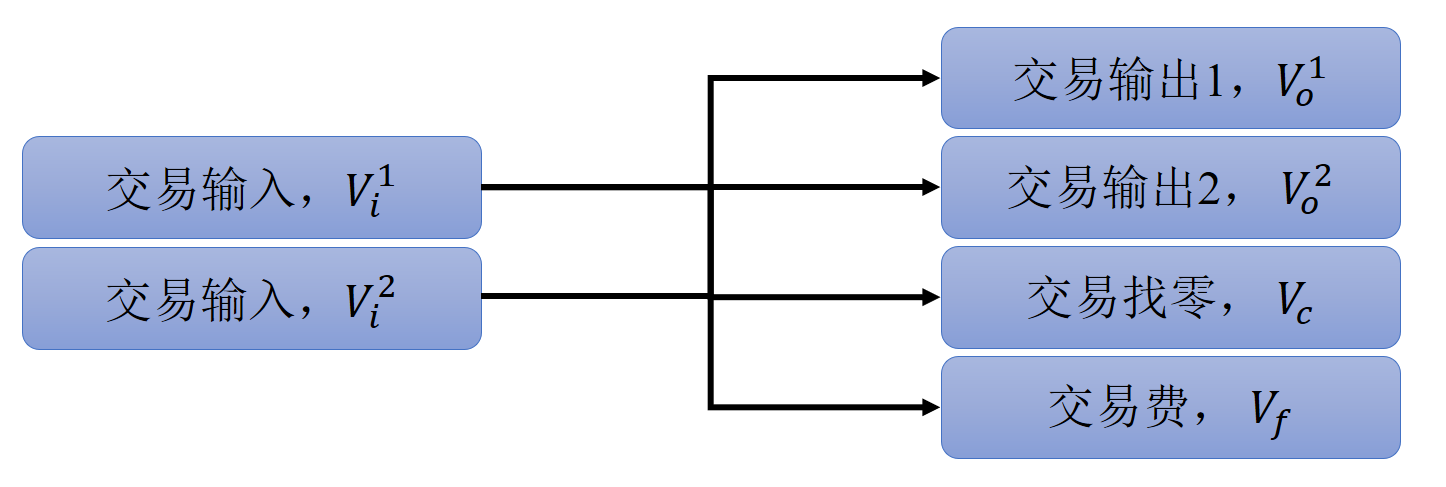
\includegraphics[width=0.75\textwidth]{figures/transaction.png}
    %\vspace{-0.1in}
    \caption{数字货币的交易流程}
    \label{fig:transaction}
\end{figure}

我们在这里给出数字货币交易的常见流程,如图\ref{fig:transaction}所示。
交易会包含至少一个交易输入$V_i$,同时对应若干个输出$V_o, V_c, V_f$。
其中$V_o$是正常交易输出;$V_c$是交易后剩余的找零,返回自己的账户;$V_f$是矿工交易费,
用于奖励矿工将这个交易打包至区块链中。在交易中,验证者需要确认交易的输入和交易的各项输出总和相等,
这样才能防止异常交易。当交易金额都是明文时,这个验证非常简单,
只需要普通加减法就可以验证。而当我们将实际交易金额都隐匿了以后,
想要验证这笔交易是否合法就困难了许多。

\section{零知识证明}

零知识证明最早由Goldwasser等人提出\cite{goldwasser1989knowledge}。
零知识证明是证明者向验证者证明某命题的方法,特点是证明过程中除``该命题为真''的事实以外,
证明者不会向验证者泄露任何资讯。普通的想向别人证明自己拥有该知识只需要对别人公开此知识内容即可,
但是这样会导致别人也知道了该知识,对自己造成损失。此时必须使用零知识证明才能在保护知识的同时,
让验证者相信证明者拥有该知识。

零知识证明可以如下形式化的定义:

\begin{itemize}
    \item 完备性:使用该证明方法,诚实的证明者确实可以向诚实的验证者证明自己持有知识。
    \item 健全性:使用该证明方法,不诚实的证明者,即未持有知识的证明者,
    能够向诚实的验证者证明自己持有该知识的概率可以忽略。
    \item 零知识:使用该证明方法证明完成后,验证者不能从中获取关于该知识的任何信息,
    也不能通过此次证明交互的内容假装成证明者,向别人证明自己或者证明者持有该知识。
    具体来说,将证明者和验证者交互的信息记录下来,由于完备性,
    任何人都能验证交互记录的合法;同时,任何不持有知识的人都能够伪造一份可以验证为合法的交互记录。
    这样说明了交互记录来自于所有可能的合法交互记录之一,和随机伪造的交互记录无法区分,
    因此没有从中透露任何信息。
\end{itemize}

\begin{figure}
    \centering
    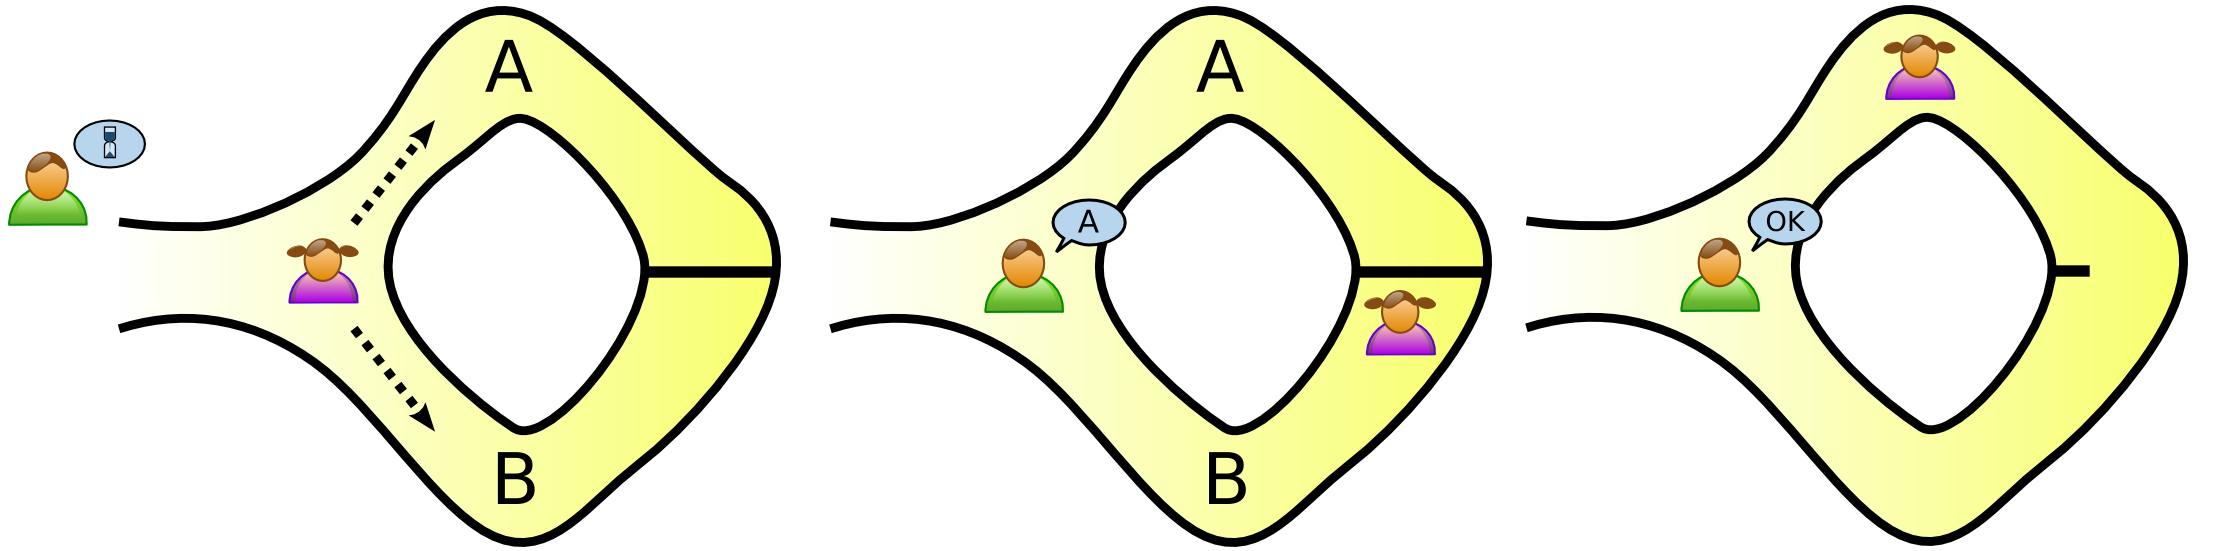
\includegraphics[width=\textwidth]{figures/alibaba.png}
    %\vspace{-0.1in}
    \caption{和零知识证明相关的寓言故事\cite{wikipedia_2021}}
    \label{fig:alibaba}
\end{figure}

对于零知识证明有一个形象的预言故事:在一座山中存在两条路,这两条路都没有岔路,
路的终点是同一扇门,如图\ref{fig:alibaba}所示。如果不打开这扇门就没法从一条路走到另一条路。
打开这扇门需要知道开门的密语,小红知道开门的密语,并且想向小绿证明这一点,
同时不想让小绿知道开门的密语。小绿需要先闭眼,让小红随机走一条路。
之后小绿告诉小红他选择的一条路,如果小红从他选择的路走回来了就算此次验证成功。
小绿和小红之间会进行很多次交互,如果小红每次都能从小绿指定的道路走回来,
那小绿就可以相信小红确实能够开门,同时小红也没有向小绿泄露开门的密语。

从零知识证明的定义分析,如果小红确实能开门,那么小红每次都能以100\%的概率从小绿指定的路回到路口,
这说明了该证明的完备性。而如果小红没有办法开门,那么每次小红都只有50\%的概率能够从指定路口回来,
只要交互次数达到了目标,小红能够通过证明的概率就可以忽略,说明了该证明的健全性。
最后,在这次证明中,小绿没有获得关于密语的任何信息,这从两方面说明。
首先小绿不能向任何人证明自己拥有该知识,由于小绿不知道密语,如果他向小黄证明,
由于小黄选择的随机道路和小绿可能不同,小绿无法利用和小红证明的过程帮助自己通过证明。
其次,小绿将该证明过程展示给其他人看时,例如将过程录制后再公开给小黄,
由于如果小红和小绿互相串通好了,实际上在证明开始前小红就知道了小绿的选择的话,
不论能不能打开门小红都能从小绿指定的道路走回来,
因此小黄不能通过这次证明过程就确定小红持有该密语。
该寓言故事中很重要的一点是小绿不能看到小红最开始是从哪条道路走的。如果小绿看到小红从道路A走,
那么他只要让小红从道路B走回来就说明小红持有密语,并且也无从得知密语;
但是这会导致该证明过程拿给任何人看都能让人推测出小红知道密语的事实,
因此也不算做零知识证明。

根据上述零知识证明的定义,结合交易金额隐匿的最终目标,
一个基于零知识证明的交易金额隐匿方法需要做到:

\begin{enumerate}
    \item 对于交易双方,可以查看交易的具体金额以及交易对象。
    这样才能够验证交易发起者确实完成了交易。
    \item 对于验证者,可以验证交易金额合法。这样保证了不会产生错误交易而导致凭空产生资金,
    同时却无法知道实际的交易金额。
\end{enumerate}

根据上述要求,在第\ref{chap:pedersen}章我们介绍数字总和承诺技术,
在第\ref{chap:bulletproof}章介绍数字范围证明技术。利用这两个技术,
验证者就能够验证交易输入和输出的数字总和相同,同时每个数字都在合法范围内。
同时交易双方通过约定承诺使用的遮罩数字,就可以查看实际的交易金额。

\chapter{数字总和承诺}\label{chap:pedersen}

为了在隐藏交易金额的同时能够验证交易金额的合法性,我们需要使用数字总和承诺的方法。
使用数字总和承诺,我们就能保证在不知道交易具体金额的情况下,
仍然能够验证一笔交易的输入金额和输出金额是相等的,
也就是这笔交易没有凭空创造出数字货币。

我们首先在\ref{sec:commit}节介绍什么是承诺,然后在\ref{sec:pedersen}节介绍Pedersen承诺,
最后在\ref{sec:amount}节说明如何进行数字总和承诺。

\section{承诺}\label{sec:commit}

一个密码学上的承诺是一种不泄露数值的情况下声明自己拥有的某个数值的方法。
一个常见的承诺方式是哈希值承诺,例如在拍卖行提交报价时,
为了防止自己的报价被其他人窃取,可以将自己报价的哈希值公开。
之后统一展示报价时,大家只要计算展示报价的哈希值是否和公开的哈希值相同即可验证报价是否成立,
同时由于哈希函数的困难特性,我们在公开哈希值后再修改报价的概率是可忽略的。
通过哈希值承诺,我们可以在不泄露真实内容的情况下让大家相信我们已经完成出价的事实。

在数字货币交易中,我们也可以使用承诺做到对交易金额的隐藏。
我们可以对交易金额加密,同时使用非对称加密技术将加密金额的密钥传递给接收者。
这样我们就无法修改伪造数值,同时接收者仍然可以验证收到的金额。

\section{Pedersen承诺}\label{sec:pedersen}

利用承诺,我们可以做到对数值的隐藏,但是验证者需要保证该交易合法,
所以在交易金额被隐藏后仍然还需要有一套机制来保证交易的合法性。
Pedersen承诺\cite{noether2016ring}就是这样一种承诺。一种承诺方案$\mathcal{H}$被叫做Pedersen承诺需要满足加法同态性,即:
%
$$\mathcal{H}(a)+\mathcal{H}(b)=\mathcal{H}(a+b)$$
%
那么我们就能够利用承诺的结果验证交易的真实性。

实际上,许多被区块链采用的哈希方案,例如离散对数、椭圆曲线方法,恰好都满足Pedersen承诺,
我们可以利用这些方法对交易金额进行承诺。需要注意的是,加密货币一般都包含小数,
而这些方法都是基于整数的,所以在加密货币实际交易时,
使用的是加密货币的最小单位为1,而不是一个加密货币为单位。
在接下来的计算中,我们使用椭圆曲线作为承诺方案,该椭圆曲线的单位元为$G$。
进行承诺时,我们会使用一个椭圆曲线上的点$H=\lambda G$,
记该承诺的公式为$C_x=\mathcal{H}(V_x)=V_xH$。

需要注意的是,如果只是简单的使用椭圆曲线等方法,还会碰到查表破解的问题。
例如我交易了$V=10^8$最小单位的加密货币,使用承诺$\mathcal{H}$得到了一个$V$的承诺$C=\mathcal{H}(V)$。
但是由于在$H$固定时任何$V=10^8$的承诺都是不变的,只要我遍历$\mathcal{H}(x)$,
我就能查表得到真实交易金额。为了避免这种情况,
在下一节我们还会引入遮盖方法,避免真实交易金额被查表得到。

\section{数字总和承诺}\label{sec:amount}

如果我们使用一个Pedersen承诺$H$,参考图\ref{fig:transaction}的交易,我们只需要验证:
%
$$C_i^1 + C_i^2 = C_o^1 + C_o^2 + C_c + C_f$$
%
就能知道交易金额是正确的了。

但是如前一节所述,如果只是直接使用椭圆曲线,我们可以查表得到承诺前的金额。
为了避免该金额被查到,我们对承诺方案加入遮罩参数。我们规定新承诺计算的公式为
$C_x=\mathcal{H}(r,V_x)=rG + V_xH$,其中$r$是一个随机数。
由于遮罩参数的存在,现在承诺的金额已经和随机数同分布了,
这样就无法通过查表得到被承诺金额。再根据上述验证公式,
如果验证公式能够通过,则有:
%
$$V_i^1 + V_i^2 + r_i^1 + r_i^2 = V_o^1 + V_o^2 + V_c + V_f + r_o^1 + r_o^2 + r_c + r_f$$
%
其中对于合法交易,$V$必定满足要求。而$r$是随机数,
因此我们只需要随机选取除$r_f$外其他$r$,并通过下式计算$r_f$:
$$r_f = r_i^1 + r_i^2 - \left(r_o^1 + r_o^2 + r_c\right)$$
%
就可以满足要求。在实际操作中,输入资金的$r_i$在生成它的上一笔资金中已经生成,
一般不需要重新生成,直接查询到上次生成的$r_i$即可。

通过该方式承诺后,为了能够让收款方能够检查收到的金额,同时矿工能够确认自己获得的矿工费,
在交易中我们会明文记录矿工费$V_f$,选取的选取的基准点$H$和计算得到的$r_f$。
这样矿工就能够自行计算矿工费的承诺$C_f = r_fG + V_fH$,并和其他承诺一起检查交易金额的正确性。
为了收款方能够查询自己受到款项的金额,我们还需要将交易金额遮罩参数存储下来,
共付款方和收款方查询。以$V_o^1$为例,我们可以使用非对称加密等方法,将$V_o^1$和$r_o^1$加密,
这样当且仅当拥有收款方密钥,才能够查看这笔交易的遮罩参数和真实交易金额。同时,
收款方仍然无法检查其他付款和收款的金额。



% \include{tex/exp}

\chapter{数字范围证明}\label{chap:bulletproof}

在前一章中,我们给出了基于Pedersen承诺的数字总和承诺方法,
从而在隐藏交易金额的同时,任何人都可以验证交易的合法性。
然而,单纯使用数字总和承诺是不够的,还有交易金额为负数和数字上溢的问题需要解决。

交易金额为负是一种非常直接的``偷窃''数字货币的方式。
我们可以向一个不存在的钱包支付金额为负的数字货币,
从而增加数字货币的实际流通数量。仍以图\ref{fig:transaction}中的交易为例,
假设输入金额分别为2和3,交易输出1为10,交易输出2为-8,交易找零为2,交易费为1,
我们可以发现:$2+3=10+(-8)+2+1$。这笔交易看似成立了,
真实交易输入只有5单位,而真实交易输出达到了13单位,完成了``无中生有''。
在明文存储交易金额的系统中,验证交易金额是否均为正数十分简单。
但是当交易金额变为了金额承诺,想在不泄露交易金额的情况下检查金额是否为负变得十分困难。

另一个问题则是在计算机中特有的数字上溢问题。由于计算机中表示整数的位数有限,
当数字过大时就会出现数值上溢,从而变成负数或其他很小的数字。
比特币在早期就曾经出现过类似问题,有人使用数值上溢漏洞向多个账户共转账了1844亿比特币\cite{btcoverflow},
远远超过了比特币预计的2100万发行量。这是由于比特币客户端使用int64类型计算交易的输入输出是否相等,
而没有检查交易是否溢出。比特币的最小单位1聪是$10^{-8}$比特币,
1844亿比特币金额恰好造成了上溢。因此,如何在交易金额承诺后检查金额是否过大十分关键。

为了解决上述两个问题,一种名为Bulletproofs的方法被提出\cite{bunz2018bulletproofs}。
该算法提出了一种零知识的数字范围证明方法,相比其他范围证明方法需要更小的交互信息量,
同时还支持在不大幅增加信息量的情况下同时证明多个数字的范围,
非常适合用于数字货币交易的范围证明中。

\section{向量内积承诺}

Bulletproofs证明基于向量内积承诺\cite{bootle2016efficient}这种承诺方案。
该承诺方案中,证明者保有两个秘密向量$\boldsymbol{a}$和$\boldsymbol{b}$,
证明者需要在不泄露这两个向量的情况下,向验证者证明这两个向量的内积为$c$,即
$\boldsymbol{a}\cdot\boldsymbol{b}=c$。

在下面的证明中,不失一般性,我们假设两个向量的长度$n$为2的幂次,
如果长度不满足条件则通过在向量后补0完成。将该证明方案记为$(G,\boldsymbol{g},\boldsymbol{h},A,B,c,n;\boldsymbol{a},\boldsymbol{b})$。
其中$G$是单位点;$\boldsymbol{g}$和$\boldsymbol{h}$是长度和$\boldsymbol{a},\boldsymbol{b}$相同,
均为椭圆曲线上的随机点,且验证者不知道这些点是单位点$G$的多少倍;$A=\boldsymbol{g}^{\boldsymbol{a}}, B=\boldsymbol{h}^{\boldsymbol{b}}$;
$c=\boldsymbol{a}\cdot\boldsymbol{b}$;$n=|\boldsymbol{a}|$;
$\boldsymbol{a},\boldsymbol{b}$为仅证明者知道的秘密向量。
除了$\boldsymbol{a},\boldsymbol{b}$,其余参数均公开。

向量内积承诺是一个交互式证明,且分为多个阶段。在每个阶段,当$n>1$时,
执行过程1,否则执行过程2。为了简便,我们使用P代表证明者,V代表验证者,
箭头表示谁向谁发送数据。

\textbf{过程1:}
\begin{enumerate}
    \item P构造以下数据:
    
    将所有向量分成两部分等长向量,即:$(\boldsymbol{g}_1, \boldsymbol{g}_2) = \boldsymbol{g}; (\boldsymbol{h}_1, \boldsymbol{h}_2) = \boldsymbol{h}; (\boldsymbol{a}_1, \boldsymbol{a}_2) = \boldsymbol{a}; (\boldsymbol{b}_1, \boldsymbol{b}_2) = \boldsymbol{b}$。
    
    此时有:$A=\boldsymbol{g}_1^{\boldsymbol{a}_1}\boldsymbol{g}_2^{\boldsymbol{a}_2},B=\boldsymbol{h}_1^{\boldsymbol{b}_1}\boldsymbol{h}_2^{\boldsymbol{b}_2},c=\boldsymbol{a}_1\cdot\boldsymbol{b}_1+\boldsymbol{a}_2\cdot\boldsymbol{b}_2$。
    
    考虑两个函数$f_a(X)=\boldsymbol{a}_1X + \boldsymbol{a}_2X^2, f_b(X)=\boldsymbol{b}_1X^{-1} + \boldsymbol{b}_2X^{-2}$,
    可以发现$f_a(X) \cdot f_b(X)$的常数项值为$c$。此时我们取随机数$x$,令$\boldsymbol{a}'=f_a(x), \boldsymbol{b}' = f_b(x), \boldsymbol{g}'=\boldsymbol{g}_1^{x^{-1}}+\boldsymbol{g}_2^{x^{-2}},\boldsymbol{h}'=\boldsymbol{h}_1^{x}+\boldsymbol{h}_2^{x^{2}}$。
    
    此时计算$\boldsymbol{g}'^{\boldsymbol{a}'}$,我们可以发现根据幂次为$x^{\{-1, 0, 1\}}$,
    可以将底数分为三组。我们将三组底数分别记为$A_{\{-1, 0, 1\}}$。
    同理计算$\boldsymbol{h}'^{\boldsymbol{b}'}$,并用$B_{\{-1, 0, 1\}}$表示底数,
    拆分两式后则有:
    
    $$A_{-1}=\boldsymbol{g}_2^{\boldsymbol{a}_1}, A_0=\boldsymbol{g}_1^{\boldsymbol{a}_1}\boldsymbol{g}_2^{\boldsymbol{a}_2}=A,A_1=\boldsymbol{g}_1^{\boldsymbol{a}_2}$$
    $$B_{-1}=\boldsymbol{h}_1^{\boldsymbol{B}_2}, B_0=\boldsymbol{h}_1^{\boldsymbol{b}_1}\boldsymbol{h}_2^{\boldsymbol{b}_2}=B,B_1=\boldsymbol{h}_2^{\boldsymbol{b}_1}$$
    
    最后$c'=\boldsymbol{a}'\cdot\boldsymbol{b}'=c_{-1}x^{-1}+c_0+c_1x, c_{-1}=\boldsymbol{a}_1\cdot\boldsymbol{b}_2,c_0=\boldsymbol{a}_1\cdot\boldsymbol{b}_1+\boldsymbol{a}_2\cdot\boldsymbol{b}_2=c,c_1=\boldsymbol{a}_2\cdot\boldsymbol{b}_1$。
    
    记$A'=\boldsymbol{g}'^{\boldsymbol{a}'}, B'=\boldsymbol{h}'^{\boldsymbol{b}'}$,
    可以看到我们基于当前的向量内积承诺证明可以构造一个新的,向量长度仅为原来一半的向量内积证明。
    如果新的证明能够通过,那说明当前的证明也能够通过。
    
    \item P$\to$V:发送$A_{-1, 0, 1}, B{-1, 0, 1}, c{-1, 0, 1}$。注意到$A_0, B_0, c_0$之前已经发送过,
    在减少数据传输的情况下可以不再发送。
    
    \item V$\to$P:一个随机数x。
    
    \item 此时,P和V分别根据收到的参数构造新的一个向量内积证明问题:
    
    $$(G,\boldsymbol{g}',\boldsymbol{h}',A',B',c',\frac{n}{2};\boldsymbol{a}',\boldsymbol{b}')$$
    
    其中新参数分别如下计算:
    
    $$\boldsymbol{g}'=\boldsymbol{g}_1^{x^{-1}}+\boldsymbol{g}_2^{x^{-2}}$$
    $$\boldsymbol{h}'=\boldsymbol{h}_1^{x}+\boldsymbol{h}_2^{x^{2}}$$
    $$A'=\boldsymbol{g}'^{\boldsymbol{a}'}$$
    $$B'=\boldsymbol{h}'^{\boldsymbol{b}'}$$
    $$c'=c_{-1}x^{-1}+c_0+c_1x$$
    $$\boldsymbol{a}'=\boldsymbol{a}_1x+\boldsymbol{a}_2x^2$$
    $$\boldsymbol{b}'=\boldsymbol{b}_1x^{-1}+\boldsymbol{b}_2x^{-2}$$
    
    就构造成了一个新的向量内积证明问题,但是向量长度减小了。之后进行下一阶段,
    求解新的向量内积证明问题。
\end{enumerate}

\textbf{过程2:}
\begin{enumerate}
    \item P$\to$V:发送当前的$(a,b)$
    \item V$\to$P:计算$A=g^a, B=h^b, c=ab$。若三式均成立则接受该证明,否则拒绝该证明。
\end{enumerate}

由于$\boldsymbol{g}$和$\boldsymbol{h}$都是验证者未知的随机取的点,
因此验证者无法在该过程中对向量的真实值进行还原。同样,因为每次验证的$x$都是验证者随机选取的,
如果证明者未持有对应向量,就无法对任意$x$给出证明。

\section{Bulletproofs证明}

Bulletproofs证明是一种基于向量内积承诺证明来完成范围证明的方案。
由于负数在计算机中使用二进制表示等价于首位为1的正数,即十分巨大的正数,
因此和数字上溢问题一样,只要保证交易金额不是过大即可。
在Bulletproofs中,我们尝试证明一个交易金额可以表示为若干2的幂次之和。
以比特币为例以其最小单位聪,即$10^{-8}$比特币来计算,
比特币共计$2.1\times10^{15}$,即只需要51位即可表示。因此,对于交易中声明的交易金额$v$,
我们只要证明$v\in[0, 2^{51}-1]$即可证明该交易金额合法。

结合前一章我们对交易金额做出了承诺,我们将范围证明做如下定义:
$v$是真实交易金额,$V=rH + vG$是该交易金额使用遮盖参数$r$的承诺。
证明者需要向验证者证明其交易金额满足$v\in[0,2^n-1]$。在该过程中,
我们可以公开$G, H, V, n$,但是需要保密$v, r$。

我们使用$a=v\{0,1\}^n$为$v$表示成二进制数时每个比特位的值组成的向量。
显然,$\langle a, I_2^n\rangle=v$,其中$I_j^n=(j^0, j^1, j^2, \dots, j^{n-1})$,
并特别规定$j=0$时第一项为0。
同时我们还需要保证$a$中元素均为1,我们通过计算新的一个向量$a_R=a-I_1$,
且$a\cdot a_R=I_0$来保证。

可以看到,目前有两个不同的约束来保证$a$是由01组成的,且是$v$的二进制表示的一个向量。
为了利用向量内积证明,我们将其改造成使用一个向量内积证明就可以的形式。
我们可以发现,如果我们想证明一个向量$k=I_0$,我们只需要让验证者发送一个随机数$l$,
并由证明者使用内积承诺证明$\langle k, l^n\rangle=I_0$即可。因为如果$k$不全为0,
那么对于任意随机数,能够通过验证的概率是可忽略的。这听起来很多此一举,
但是利用这种方法我们将一个向量内容的证明问题转换为了使用内积承诺来证明,
这使得我们可以将元素均为1中构造的两条公式转为向量内积承诺的形式。
在收到验证者指定的随机数$y$后,我们有:
%
$$a_R=a-I_1 \to a - a_R - I_1 = I_0 \to \langle a - a_R - I_1, y^n\rangle=0$$
%
$$a\cdot a_R=I_0 \to \langle a, a_R \cdot y^n\rangle=0$$
%
第一个公式使用了上述结论。第二个公式也很显然,对其中一边的向量放大若干倍,其内积依然为0。

此时验证者再提供一个新的随机数$z$,我们可以将上述两个式子和最开始的值相等式子组合得到:
%
$$z^2\cdot\langle a, I_2\rangle + z\cdot\langle a - a_R - I_1, y^n\rangle + \langle a, a_R \cdot y^n\rangle=z^2\cdot v$$

此时我们可以对该式子的左右分别求和,然后问题就转化成了一个标准的向量内积问题。
我们将在之后解决证明中的隐私泄露问题,即证明中不能明文利用到$v, a, a_R$。

我们将上式展开,并在左右同一加上$\langle -z\cdot I_1, z^2\cdot I_2 + z\cdot y^n\rangle$,
然后化简。需要注意,$y^n=y^n\cdot I_1, \langle a_R, y^n\rangle = \langle I_1, a_R\cdot y^n\rangle$,得到:
%
$$\langle a - z\cdot I_1, y^n(a_R + z\cdot I_1) + z^2\cdot I_2\rangle = z^2\cdot v + (z - z^2) \langle I_1, y^n\rangle - z^3\langle I_1, I_2\rangle$$

此时,问题已经转化为了一个可以使用向量内积问题证明的问题。
在完成转换后,我们使用向量内积证明的方式进行计算,如果证明者证明了向量内积的承诺和$v$的承诺相等,
就证明了$v$的范围是在给定范围内的。然而,此时左侧向量$a - z\cdot I_1$求得的$A$可以简单推算出$v$,
因此还需要一步遮盖方法。我们使用遮盖向量$s, s_R$对$a, a_R$进行遮盖。
验证者会随机给出多个随机数$X$,上式的左右向量分别变为:

$$
\begin{array}{l}
l(X)=\left(a+s \cdot X\right)-z \cdot I_1  \\
r(X)=y^n \cdot\left(\left(a_{R}+s_{R} \cdot X\right)+z \cdot I_1\right)+z^{2} \cdot I_2  \\
t(X)=\langle l(X), r(X)\rangle=t_{0}+t_{1} \cdot X+t_{2} \cdot X^{2} 
\end{array}
$$

此时经过遮盖,向量已经不会泄露原始信息。由于包含遮盖的项必定包含$X$,
此时,我们需要证明$t_0$和之前等式右边的结果相同。同时,证明$t(X)=\langle l(X), r(X)\rangle$,
且$l(X), r(X)$均成立。因此,证明者可以通过提前承诺$t_1$和$t_2$,
然后在每次获取随机数$x$时生成$l(x), r(x)$,并通过向量内积承诺计算这两个向量的内积。
验证者需要验证这两个向量的内积,结合之前给出的$V, t_1, t_2$的承诺计算得到的$t(x)$是否相等。
至此,我们可以通过Bulletproofs方法对一个数字的范围进行证明。

然而,一笔交易中包含很多的数字,如果要对每个数字都进行一次范围证明代价较大。
注意到在Bulletproofs中实际上将所有数字使用二进制表示来完成证明,
我们可以将所有数字的二进制表示串连起来,这样通过一次证明即可完成所有数字的范围证明。
例如有两个数字$a^0, a^1$,我们需要证明所有数字都满足$a\in[0, 7]$,
那么我们可以造下面两个向量和内积:
%
$$A=\langle a^0_0, a^0_1, a^0_2, a^0_3, a^1_0, a^1_1, a^1_2, a^1_3 \rangle$$
%
$$B = \langle 0, 1, 2, 4, 0, 1, 2, 4\rangle$$
%
$$c=a^0 + 8 a^1$$
%
就可以通过一次证明完成。由于向量内积承诺进行的轮数与向量长度相关,
对于长度为$n$的向量其证明复杂度为$O(log_2n)$,相比每个数字依次证明的复杂度$O(mlog_2n)$,
这种证明方式的复杂度下降为$O(log_2nm)$。


\begin{comment}
\begin{figure}
    \centering
    \includegraphics[width=46mm]{images/placeholder.png}
    %\vspace{-0.1in}
    \caption{123}
\end{figure}


\begin{figure}
    \centering
    \includegraphics[width=46mm]{images/placeholder.png}
    \includegraphics[width=23mm]{images/placeholder.png}
    %\vspace{-0.1in}
    \caption{456}
\end{figure}
\end{comment}

% 后置部分包含参考文献
\backmatter

% 打印参考文献列表
\printbibliography

\end{document}
